\documentclass[conference]{IEEEtran}
\IEEEoverridecommandlockouts
% The preceding line is only needed to identify funding in the first footnote. If that is unneeded, please comment it out.
\usepackage{cite}
\usepackage{amsmath,amssymb,amsfonts}
\usepackage{algorithmic}
\usepackage{graphicx}
\usepackage{textcomp}
\usepackage{xcolor}
\usepackage{float}
%\restylefloat{table}
\def\BibTeX{{\rm B\kern-.05em{\sc i\kern-.025em b}\kern-.08em
    T\kern-.1667em\lower.7ex\hbox{E}\kern-.125emX}}
\begin{document}

\title{Data-Driven Admissions in Education: Enhancing Student Success by Matching Profiles to Optimal Academic Paths\\
{\footnotesize \textsuperscript{}}
\thanks{}
}

\author{\IEEEauthorblockN{Clément Combier}
\IEEEauthorblockA{\textit{Master 2 SIGLIS} \\
\textit{Université de Pau et des Pays de l'Adour}\\
Anglet, France \\
clement.combier@etud.univ-pau.fr}}
\maketitle

\section*{abbreviation}
\begin{itemize}
    \item[] AI : Artificial Intelligence
    \item[] ML : Machine learning
    \item[] KNN : K-Nearest Neighbors
    \item[] CNN : Convolutional Neural Networks 
    \item[] RNN Recurrent Neural Networks 
    \item[] SVM : Support Vector Machines 
    \item[] RF : Random Forest
    \item[] SMOTE : Synthetic Minority Oversampling TEchniques
\end{itemize}


\vspace{16pt}

\begin{abstract}
In the wake of the COVID-19 pandemic and the release of the new \textit{baccalaureate} reform, French education authorities in higher studies faces a surge of enrolments and higher dropouts numbers. Higher grade from students in the baccalaureate as lead, the French registration system in place to accept more and more students in higher degrees paths. Sadly, these new reforms did not take into account the difficulty step created between secondary and higher studies. Thus augmenting the number of dropouts in students who don't have the capacity, motivation and/or will to continue in their path. 

We propose a solution to mitigate this dropout as well as helping academia to find \textit{excellence students} with compatible profile for a certain path (diploma and domain). Taking the problem at its root could lead to a \textit{two birds with one stone} resolution to the problem.

This paper focuses on critical issues within the education system and tries to differ a more holistic and personalized approach to student placement. By using data mining, analytic and machine learning, we hope to create a more harmonious and productive education landscape for both students and academic alike.
\end{abstract}
\vspace{8pt}
\begin{IEEEkeywords}
Higher education, Admission process, Machine learning, Data analytics, Success rate, Dropout rate, Student profile, Optimization, Profile-degree matching, Admission management, High-achieving students, Adaptive education.
\end{IEEEkeywords}
\vspace{16pt}

\section{Introduction}
Today education landscape in higher education is rapidly evolving due to higher levels of education and possibly COVID-19, the surge in higher education enrolment presents new challenges : how to manage increasing number of admissions and how to ensure academic success. 
An estimated 2.97 million students registering for higher education in France for the year 2021-2022, marking a 2.5\% increase from the previous year \cite{sous-direction_des_systemes_dinformation_et_des_etudes_statistiques_sies_les_2022}. Globally, UNESCO reported a rise from 28.5 million students in 1970 to an estimated 235 million in 2023 \cite{unesco_higher_2023}.

However, this increase in enrolment has not necessarily translated into higher success rates. As illustrated in Table \ref{tab:result_bachelor}, the cumulative success rate over 4 years for students enrolled in Bachelor's programs in France remains a concern, with only 39.8\% of the 2010 cohort succeeding by 2014.

\begin{table}[H]
    \centering
    \caption{Results in Bachelor's degree for the 2013 and 2014 sessions for students enrolled for the first time in the first year of Bachelor's in 2010-2011.\cite{kabla-langlois_insee_2016}}
    \begin{tabular}{|c|c|}
        \hline
        \textbf{Headcount 2010} & \textbf{Cumulative success over 4 years (in \%)}\\
        \hline
        169 652 & 39.8 \\
        \hline
    \end{tabular}
    \label{tab:result_bachelor}
\end{table}

In France, the Parcour sup system was introduced to manage the influx of candidates and match them with suitable programs. Despite its intentions for uniformity and transparency, it has faced criticism for not adequately addressing the mismatch between student potential and program suitability, which is a contributing factor to the low success rates \cite{couto_parcoursup_2021}.

But what can be categorized as student success, and how to tell if a student enters the profile of excellence? Most of the time, success is, for institute, the number of student who graduate their degree. \cite{weatherton_success_2021}. However, even if this correlation can indicate a good rate of success for an institute or university, is it really indicative of real success? For our research, we have chosen to stay with the simple success definition of how many students can graduate to stay within a binary model for our ML. However, to really answer the problematic of highlighting an excellent student, we will take into account other factors.
Another definition we have to pin is the definition of excellent student. By definition, it could be written like so, “an excellent student is one with good grades, a good understanding of the concepts and a general interest in the field of study.” Independent of students with ease for learning, an excellent student may not perform well in a casual course cursus, but out stand in a specific field he or she is interested in. 

This research endeavours to explore and validate the potential of ML and data analytics in revolutionizing the admission process. The motivation is twofold: to enhance the success rate of students by ensuring they are placed in programs where they are most likely to excel, and to reduce dropout rates by minimizing mismatches between students and programs. We also thrive to found more excellence students within the mass of registration.

This research will explore and proposes of different approach, starting with a detailed methodology, followed by a case study made within the University of Pau et des Pays de l'Adour. 
We will then conclude, taking into account our findings and the result of our experiment 

\section{State of the art}
\label{sec:soa}
For our subject, we delve into the optimization of finding excellence students within the mass of registration, as well as to help students find their correct path depending on their profile. This approach should theoretically reduce students dropout within higher degree studies.
We've focused our attention on using ML to predict student dropout, as it has been under heavy study within the field. From both an analytical standpoint to a predictive one using different method, algorithm, and models of ML.

We have cut our review in two big sections. The first one will explore the importance of student choice for success, then, in the second part, we will review the field of student dropout prediction using ML. This second section itself cut into two parts, the first one focusing on the analytical approach to the problem, then, in the second part, on the predictive models used to predict student dropout in the literature.

\subsection{Importance of student's choice for success in higher education}
Our first question we have to ask is if student choice really matter for the success in higher education or not. Does other factors influence this rate, does student choice influence heavily the chance of success for a student?
Multiple paper have searched the reasons behind student success to highlight the important factor to take into account.

A common recurrent topic on that subject is the lack of holistic approach by academia and researchers on the concept of student success. It is often regarded as a “common sense” where student success is measured not by the score of students, but rather how many got their diplomas. \cite{weatherton_success_2021}.

From different literature review and papers, research seems to diverge and agree on different aspects. Making it difficult to pinpoint a specific variable that could point us in the direction of success prediction. From the country to institution itself, student history and background. It seems like choice has an important effect on whether a student may be successful in its study or not. However, we cannot satisfyingly say that choice makes student success.  Some outliers may have bad grades but be in reality a high potential success student. It all depends on a myriad of factors, which can be distilled into different variable that our ML algorithms can learn from. However, we cannot use only student's choice. We have to actually see and search (as we are going to do when looking at student dropout factors), which factors can be used to feed our models in order to correctly predict student success and find these outliers within the mass.\cite{kuh_what_2006, sa_how_2018}

\subsection{Predicting student dropout}
The body of literature concerning student dropout is comprehensive, encompassing a range of perspectives from diverse academic disciplines. The issue has been approached through psychological and economic lenses, utilizing both qualitative and quantitative research methods. This section is structured to reflect the various domains and methodologies present in prior studies.

We've cut this section in two major subsections. The first one, \ref{subsec:soa_analyticalapproeach}, will review the different ways of analytical analysis on student dropout. These different approaches went from simple adaptation models to economic models and psycho-pedagogic models to predict and describe student dropout. Then, in \ref{subsec:soa_predictiveapproach} we are going to study different mathematical algorithms and models and use ML models to predict student dropout.

\subsubsection{Analytical approach}
\label{subsec:soa_analyticalapproeach}
This first part will delve inside the different perspectives of research outside the predictive fields using ML. We found these different point of view interesting to study for our future predictive model. These research have different conclusion on why students dropout from their studies, from an economical standpoint to a psychological one.
(Opazo et al. 2021)\cite{opazo_analysis_2021} have found an interesting link with the study from (Spady 1970) which found a correlation between the student dropout model and the social nature of suicide (\textit{social integration}), (Durkheim, 1951). This theory implies that the likelihood of suicide increase when there is an absence of : a)\textit{low normative congruence} and b)\textit{low friendship support}. Other literature from their state-of-the-art list these following as recurrent factors from multiple research\cite{opazo_analysis_2021}\cite{spady_dropouts_1970,tinto_dropout_1975,caspersen_teachers_2015,lidia_problema_2006,bejarano_caso_2017,sinchi_acceso_2018,cavero_voluntad_2011,velasco_alisis_nodate}: 
\begin{itemize}
    \item family
    \item previous educational background
    \item academic potential
    \item normative congruence
    \item friendship support
    \item intellectual development
    \item educational performance
    \item social integration
    \item satisfaction
    \item institutional commitment
    \item student adaptation
\end{itemize}
We can decisively take into account these factors for our study has they have been proven to be recurrent factors throughout the literature on predicting students dropout.

In another study based in South Korea, they have defined the other type of factor for students (high-school students) \cite{lee_machine_2019} :
\begin{itemize}
    \item Diseases
    \item Family Problem
    \item Poor Academic Performance
    \item Poor Relationship with Others
    \item Strict School Rules
\end{itemize}


\subsubsection{Predictive Approaches}
\label{subsec:soa_predictiveapproach}
Several researches focused on predictive approaches such as, Association rules mining, ANN based algorithm, Simple Logistic, 
 Random Forest, Logistic regression analysis, ICRM2.\cite{mduma_survey_2019}. 
In this paper, we are going to analyse the following models \cite{mduma_survey_2019}\cite{quinlan_induction_1986,yadav_mining_2012,heredia_student_2015,ramirez_prediction_2018,cox_regression_1958,perez_modelo_2018,pandey_data_2011,cover_nearest_1967,mardolkar_forecasting_2020,zhang_neural_2000,rudin_stop_2019,siri_predicting_2015,m_alban_she_is_with_the_faculty_of_engineering_and_applied_sciences_of_the_technical_university_cotopaxi_neural_2019,boser_training_1992,lee_machine_2019,behr_early_2020,friedman_stochastic_2002,eckert_analysis_2015,tenpipat_student_2020,liang_machine_2016,liang_big_2016,fischer_angulo_modelo_2012,miranda_analysis_2017,viloria_integration_2019,kemper_predicting_2020,agrusti_university_2019}:
\begin{enumerate}
\item Decision Trees
\item Logistic Regression
\item K-Nearest Neighbors (KNN)
\item Neural Networks
%\item Support Vector Machine
\item Random Forest
\end{enumerate}
From this review paper \cite{agrusti_university_2019}, we can extract this following table of these different techniques and how often they were used in other research paper.
\begin{table}[H]
    \centering
    \caption{CLASSIFICATION TECHNIQUES frequencies\cite{agrusti_university_2019}}
    \begin{tabular}{|c|c|}
        \hline
        \textbf{Techniques} & \textbf{Frequency}\\
        \hline
        Decision Tree & 49\\
        \hline
        Neural Networks & 29\\
        \hline
        Logistic regression & 25\\
        \hline
        KNN & 9\\
        \hline
    \end{tabular}
    \label{tab:class_tech_freq_agrusti}
\end{table}
These models have been chosen as they have been the most recurring ones within the literature. We will analyse each models to list the pros and cons of each one and to determine which one(s) we should use to build our predictive system.


\vspace{8pt}
\paragraph{Decision Tree}
The Decision Tree model, in ML, stand out as a fundamental and versatile algorithm. It is widely recognized for their simplicity and efficacy for classification and regression tasks alike.
Their tree-like structure gave them their name to the algorithm, comprised of nodes and branches (symbolizing decisions and their possible consequences). This helpful visualization and interpretation makes complex decision-making processes easier and intuitive for the user. This visualization is really powerful and is an invaluable tool in various applications, ranging from data mining to advanced research in AI.

Decision trees have been used in a wide range of fields such the medical, game-theory weather prediction and much more.\cite{quinlan_induction_1986}.
From the literature, decision tree seems to have a precision of around 83\% based on multiple papers (73\% \cite{viloria_integration_2019}, 87.27\% \cite{ramirez_prediction_2018}, 83\%\cite{kemper_predicting_2020} and around 90\% \cite{tenpipat_student_2020}). This research paper has evaluated multiple algorithm within decision tree and graphed out a ROC Curve for each of their algorithm. In a similar domain as this study, which is students dropout in South Korea schools and how to predict them. Their ROC curves showed that for a low rate of false positive, we get an outstanding true positive rate. Approximately attaining their limits around 0.2 false positive rate\cite{lee_machine_2019}. This study shows the predictive efficiency of the decision tree model. 
One downside of each study is the granularity of student prediction. They have shown which variable can be used to determine which kind of students may be at risk of dropout, but they lack a micro vision to alert staff about a specific student at risk.

\vspace{8pt}
\paragraph{Logistic Regression}
Logistic regression, different from linear regression by its ability to handle binary outcomes (scenarios where the outcome is dichotomous), is an important part of the statistical method in the field of ML. It is particularly interesting for its role in classification tasks. This method works by modeling the probability of a binary response, based on one or more predicator variables (independent variables). 
Our scenario of student dropout is not dichotomous by nature. However, this method can be a first step for data cleansing and classification of at risk student and out of risk students.

An interesting approach by this study \cite{lan_sparse_2014} - which change the granularity of the prediction to a student based one - is to create a “grade book” (a source of information commonly used in the context of classical test theory \cite{novick_axioms_1966}), filed with ones if the student answer correctly to question \textit{i} or 0 if not. Then, weights are added to each question depending on their difficulty to define if a student is at risk of failing and dropout. However, this approach does include some sort of e-learning method, and does solve the problem from a per-student level. Yet, it does not take into account other factors cited above to paint a bigger picture of a life of a student, and thus, defining if this student is at risk or not. It could simply be failing this course, and even if a pattern arises for a specific student (of failing), can we conclude he is at risk of dropping out?

\vspace{8pt}
\paragraph{K-Nearest Neighbors (KNN)}
K-Nearest Neighbors (KNN) is fundamental in the field of ML. As a non-parametric, instance-based learning algorithm, it is particularly renewed for its simplicity and effectiveness for tasks such as classification and regression.
The core principle of KNN is to predict labels of new data points by looking at the closest labelled data points 'K' and - for classification, take a majority vote - or an average in the case of regression. This algorithm basically learns by itself with the more data it is fed.
It can be really powerful in our case, as it excels in scenarios where the decision boundary is irregular and blurry.

The following study \cite{shiful_machine_2021}, compared to other methods, was the second most accurate models from all other models (apart from the Random Forest algorithm).
\begin{table}[H]
    \centering
    \caption{Training and testing Accuracy\cite{shiful_machine_2021}}
    \begin{tabular}{|c|c|c|}
        \hline
        \textbf{Model name} & \textbf{Training accuracy}  & \textbf{Testing accuracy}\\
        \hline
        Decision Tree & 80\% & 80\% \\
        \hline
        KNN & 83\% & 84\% \\
        \hline
        Random forest & 94\% & 86\% \\
        \hline
    \end{tabular}
    \label{tab:training_testing_acc_shiful}
\end{table}

This review shows us that, even though it  might not be the most accurate model (at least in this study \cite{shiful_machine_2021}), it is an interesting model to chose for comparing students between them, and potentially discover groupings of students which may be at risk of dropout.

From this same study, the searchers have compared each classifier for each model. For KNN, they found these results :
\begin{table}[H]
    \centering
    \caption{Comparison of all classifier\cite{shiful_machine_2021}}
    \begin{tabular}{|c|c|c|c|}
        \hline
        \textbf{Classifier} & & \textbf{Precision} & \textbf{recall}\\
        \hline
        KNN & Not Dropout & 86\% & 84\% \\
        \cline{2-4} 
        & Dropout & 69\% & 26\% \\
        \hline
    \end{tabular}
    \label{tab:compar_classifier_shiful}
\end{table}

This result implies that the model is pretty accurate, with an estimated 85\% of accuracy with these new results.

\vspace{8pt}
\paragraph{Neural Networks}
Neural network envision the AI and ML landscape by taking inspiration from the human brain's structure and function. A network is composed of layers of interconnected neurons, each capable of performing simple probability computations. Thanks to these layers of computations, a Neural Network can learn complex patterns and relationships in data from the input. This makes the incredibly powerful for a wide range of tasks. 
This technique turned into a field of its own, which now includes different structured Neural Network such as Convolutional Neural Networks (CNN) and Recurrent Neural Networks (RNN), each useful for specific types of dataset and tasks. Their learning capacity and ability make them an incredible powerful tool in the field of AI and ML. 

Neural Network is a vast field in itself. This first study used the Perceptron Multilayer algorithm with an admissible error of 0.0001 and using the hyperbolic tangent function for activating input and output layers\cite{viloria_integration_2019}. They have estimated that the classification was 83\% accurate according to the ROC curve of the neural network classifiers.
\begin{table}[H]
    \centering
    \caption{Comparison of the classifier evaluation parameters\cite{viloria_integration_2019}}
    \begin{tabular}{|c|c|c|}
        \hline
        \textbf{Model name} & \textbf{Precision}  & \textbf{Recall}\\
        \hline
        Decision Tree & 72\% & 64\% \\
        \hline
        Neural network & 73\% & 65\% \\
        \hline
    \end{tabular}
    \label{tab:comparaison_classifier_eval_param_viloria}
\end{table}

This new table of comparison of classifier per model shows us one more time that we cannot establish if one is better than the other or not. Once more, each model has is particularities, advantages, and disadvantages. 

The perceptron Multilayer algorithm is the most commonly used algorithm within the field of ML and AI.\cite{siri_predicting_2015} For this research, they have study :
\begin{quote}
    "This study asked two research questions: 
    \begin{enumerate}
        \item How accurately do pre-entry students’ characteristics predict the risk of dropout?
        \item Which characteristics weigh most in predicting the risk of dropout?"
    \end{enumerate} 
\end{quote}\cite{siri_predicting_2015}
For both question, they have concluded that the model is a pilot instrument and may be enhanced. They advised that :
\begin{quote}
    "Future research should consider the extension of the study to other groups of students not only enrolled in the healthcare area because it could reveal the importance of including additional variables not considered in this research."
\end{quote}\cite{siri_predicting_2015}

In this other study \cite{siri_predicting_2015}, their neural network model had a prediction accuracy of about 84\% for their first study group, 81\% for group 2 and 76\% for the dropout group. 

We will see in the conclusion of this literature review, which model seems to be the more fitted for our problem, taking into account the complexity and cost of each model as a system.
\vspace{8pt}
%\subsubsection{Support Vector Machine (SVM)}
%Support Vector Machines (SVM) are a powerful and versatile method for classification and regression tasks. 

%Support Vector Machines (SVM) are a powerful and versatile class of supervised learning algorithms, widely recognized for their robustness and efficacy in classification and regression tasks. Central to the SVM methodology is the concept of finding the optimal hyperplane that best separates different classes in the feature space. This is achieved by maximizing the margin between the data points of different classes, which are represented as vectors in this space. SVMs are particularly adept at handling high-dimensional data and are known for their ability to manage overfitting, even in complex datasets with a large number of features. The flexibility of SVMs is further exemplified through the use of kernel functions, which allow them to operate in a transformed feature space, enabling the handling of non-linear relationships. This makes SVMs highly effective for a wide range of applications, from text classification to bioinformatics. As we explore the current landscape of machine learning, understanding the nuances of SVMs, including their theoretical foundations, practical implementations, and the scenarios where they excel, is essential for appreciating their significant role in advancing the field of predictive modeling and data analysis.

%\textit{\textbf{W.I.P}}
%\vspace{8pt}$
\paragraph{Random Forest}
Another good method for classification and regression tasks, Random Forest, is a robust and versatile learning method. It operated by creating a multitude of decision trees during training, then outputting the class - for classification, the mode of the classes - for regression, the mean prediction (for each individual tree).
This technique enhance the predictive accuracy and overcomes the overfitting problem associated with single decision tree.
Its strength lies in its ability to handle large datasets without extensive data preprocessing requirements. 

One student focused on different Random Forest algorithm, including RF using the synthetic minority oversampling techniques (SMOTE) or Boosted RF. It showed interesting premises with from a predictive standpoint. \cite{lee_machine_2019}
\begin{table}[H]
    \centering
    \caption{AUC results of the classifiers used in this study\cite{lee_machine_2019}}
    \begin{tabular}{|c|c|}
        \hline
        \textbf{Model} & \textbf{AUC}\\
        \hline
        Random Forest & 0.986 \\
        \hline
        RF + SMOTE & 0.986\\
        \hline
        Boosted RF & 0.988 \\
        \hline
    \end{tabular}
    \label{tab:auc_values_lee}
\end{table}

Boosted RF is an advanced version of RF using boosting. Boosting is a method of sequentially improving a model's accuracy by focusing on previous models' misclassification. The algorithm starts with a base RF and iteratively adds more trees. Each new tree trained on the residuals of the previous ensemble of trees. This process continues until a specified number of trees are added, or no significant improvement is observed.

SMOTE is a powerful approach used in ML. Primarily used when dealing with imbalanced datasets (datasets where one class, usually the class of interest, is underrepresented compared to other classes). These datasets lead to poorly performing and biased models.
However, it's important to apply SMOTE carefully, as it can introduce noise into the dataset. This approach is best used with a large dataset and when the minority class is underrepresented in order to create meaningful synthetic samples.

\vspace{8pt}
\subsubsection{Conclusion}
This review has shown the multifaceted nature of the issue. The analytical approach — exploring psychological, economic, and socio-cultural dimensions — has emphasized the significance of a broad spectrum of factors. The predictive approach has demonstrated the capabilities of machine learning algorithms in identifying students at risk of dropping out, with techniques like Decision Trees, Logistic Regression, K-Nearest Neighbors, Neural Networks, and Random Forest showing varying levels of precision and applicability.
From the studies in student's dropout, we can extract interesting information to base our subject on. We could use these findings and train our machines differently to predict success and not failure.

\section{Conceptual implementation}

\begin{figure}
    \centering
    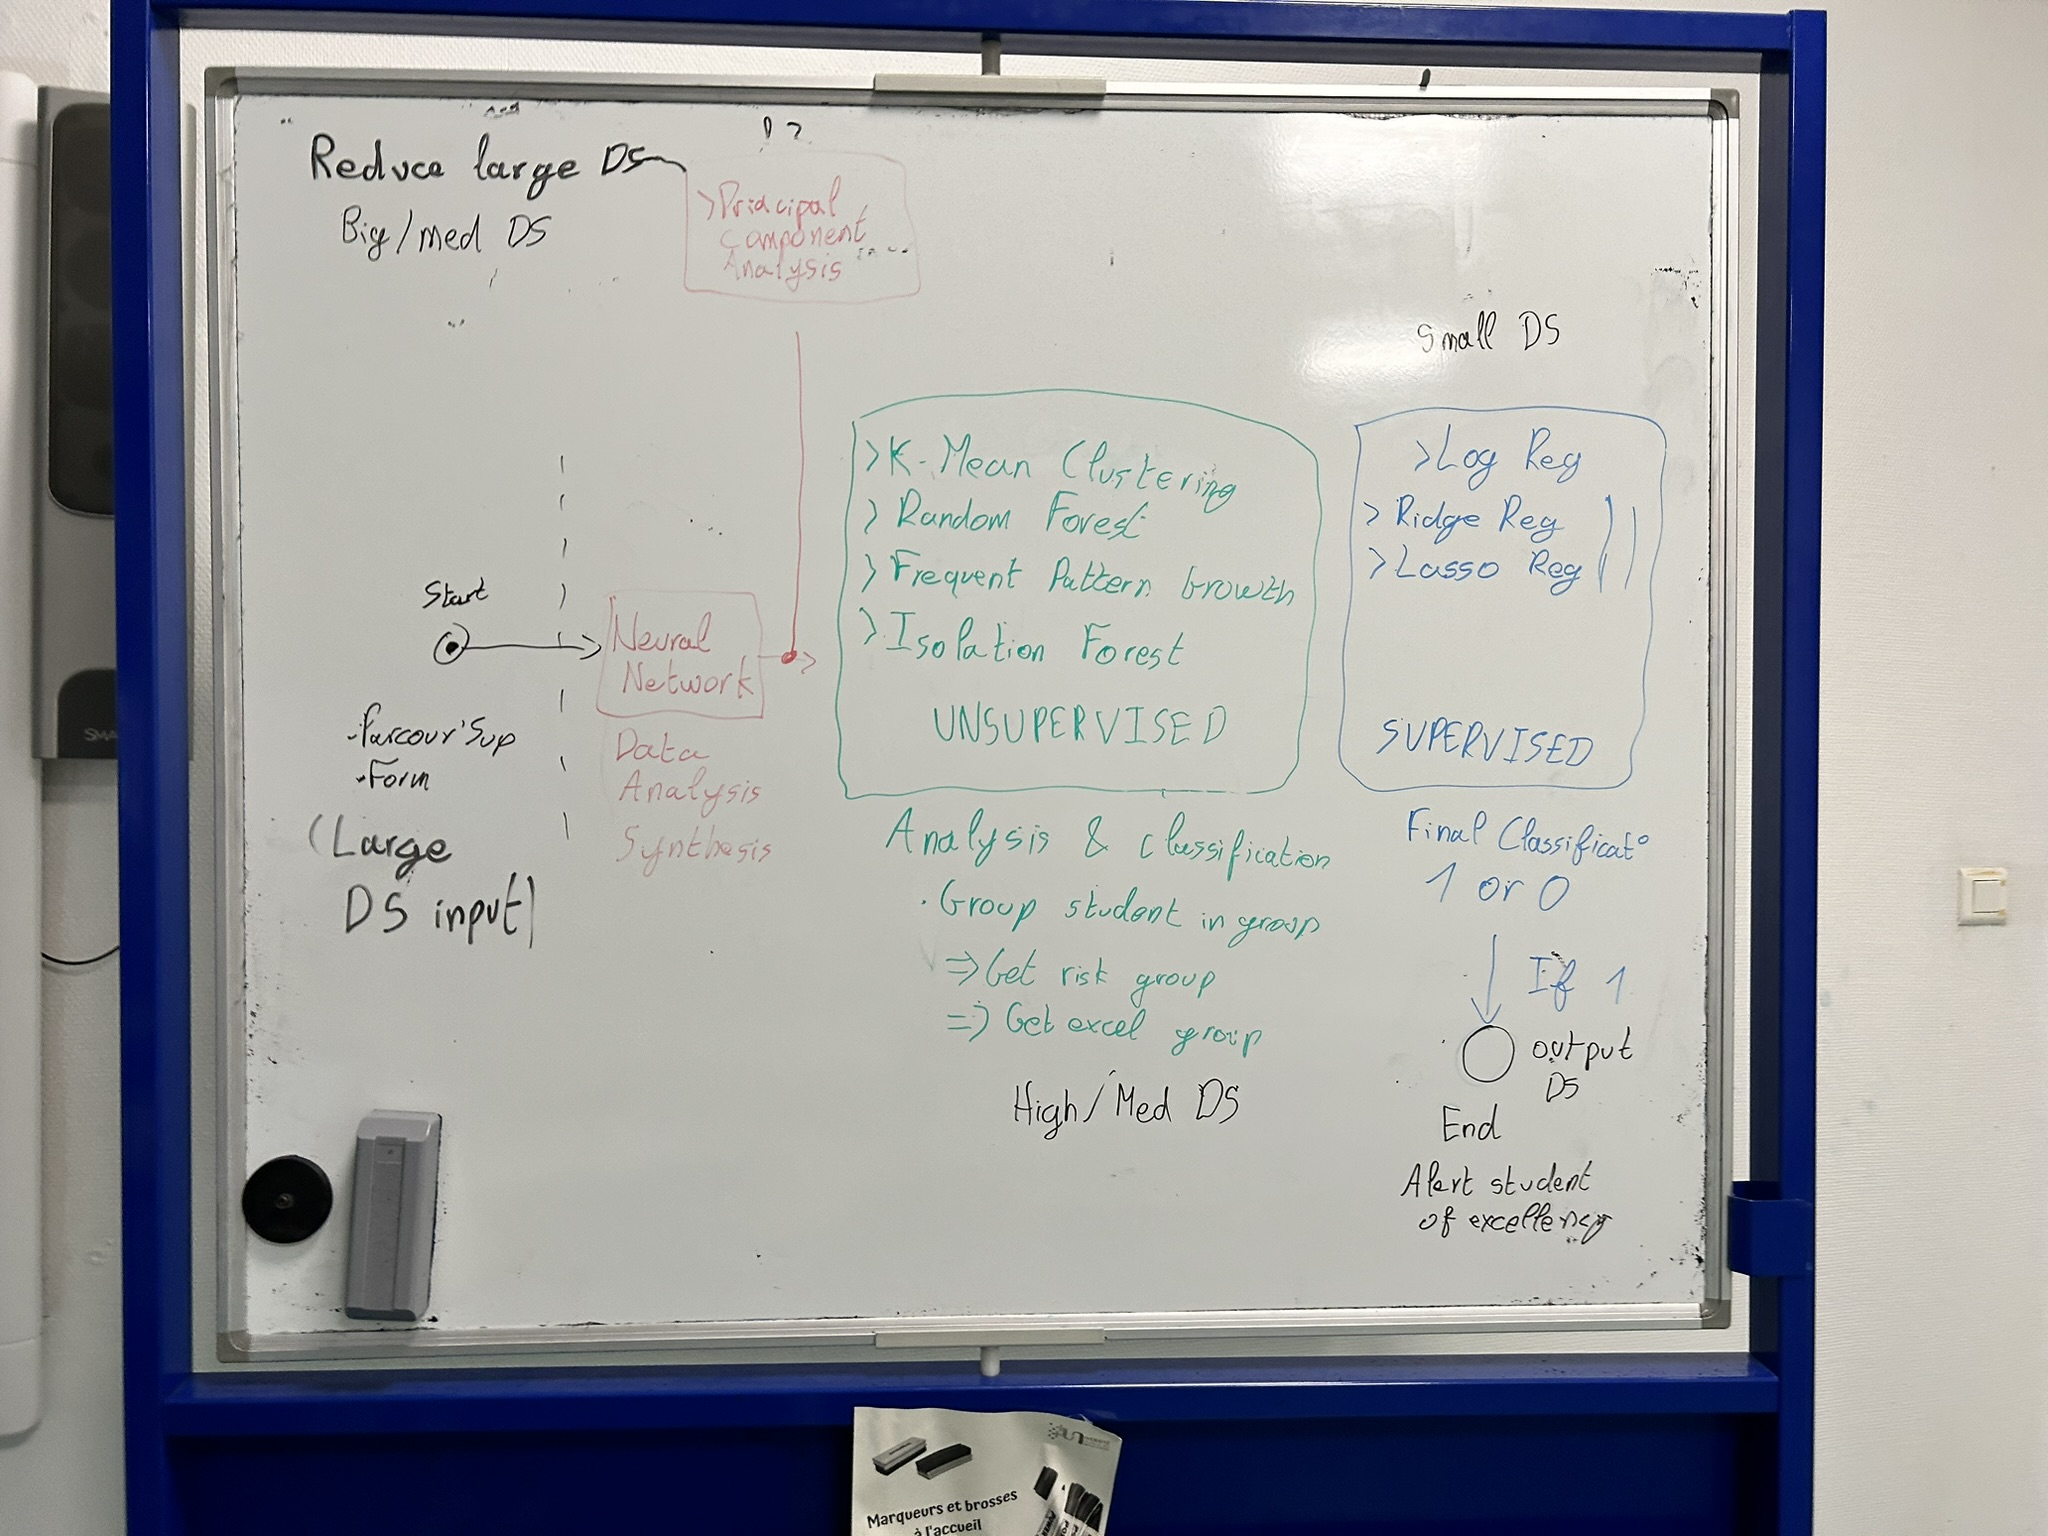
\includegraphics[width=1\linewidth]{res//diagram/approach_v1_raw.jpeg}
    \caption{Methodology mock-up v.1}
    \label{fig:enter-label}
\end{figure}

\vspace{16pt}
\section*{Acknowledgment}
\vspace{12pt}

\bibliographystyle{plain}
\bibliography{bib/references}

\end{document}
